%*----------- SLIDE -------------------------------------------------------------
\begin{frame}[t]{Introdução} 
    \transdissolve[duration=0.5]
    Field of research focused on studies in \textbf{underwater robotics}, aspects of computational dynamics, applications of basic functionalities of a robotic and search and analyze technology trends of this field.

   
    %\newline
        \begin{columns}[t]
            
            \column{0.33\linewidth}
            \begin{center}
            \begin{figure}
                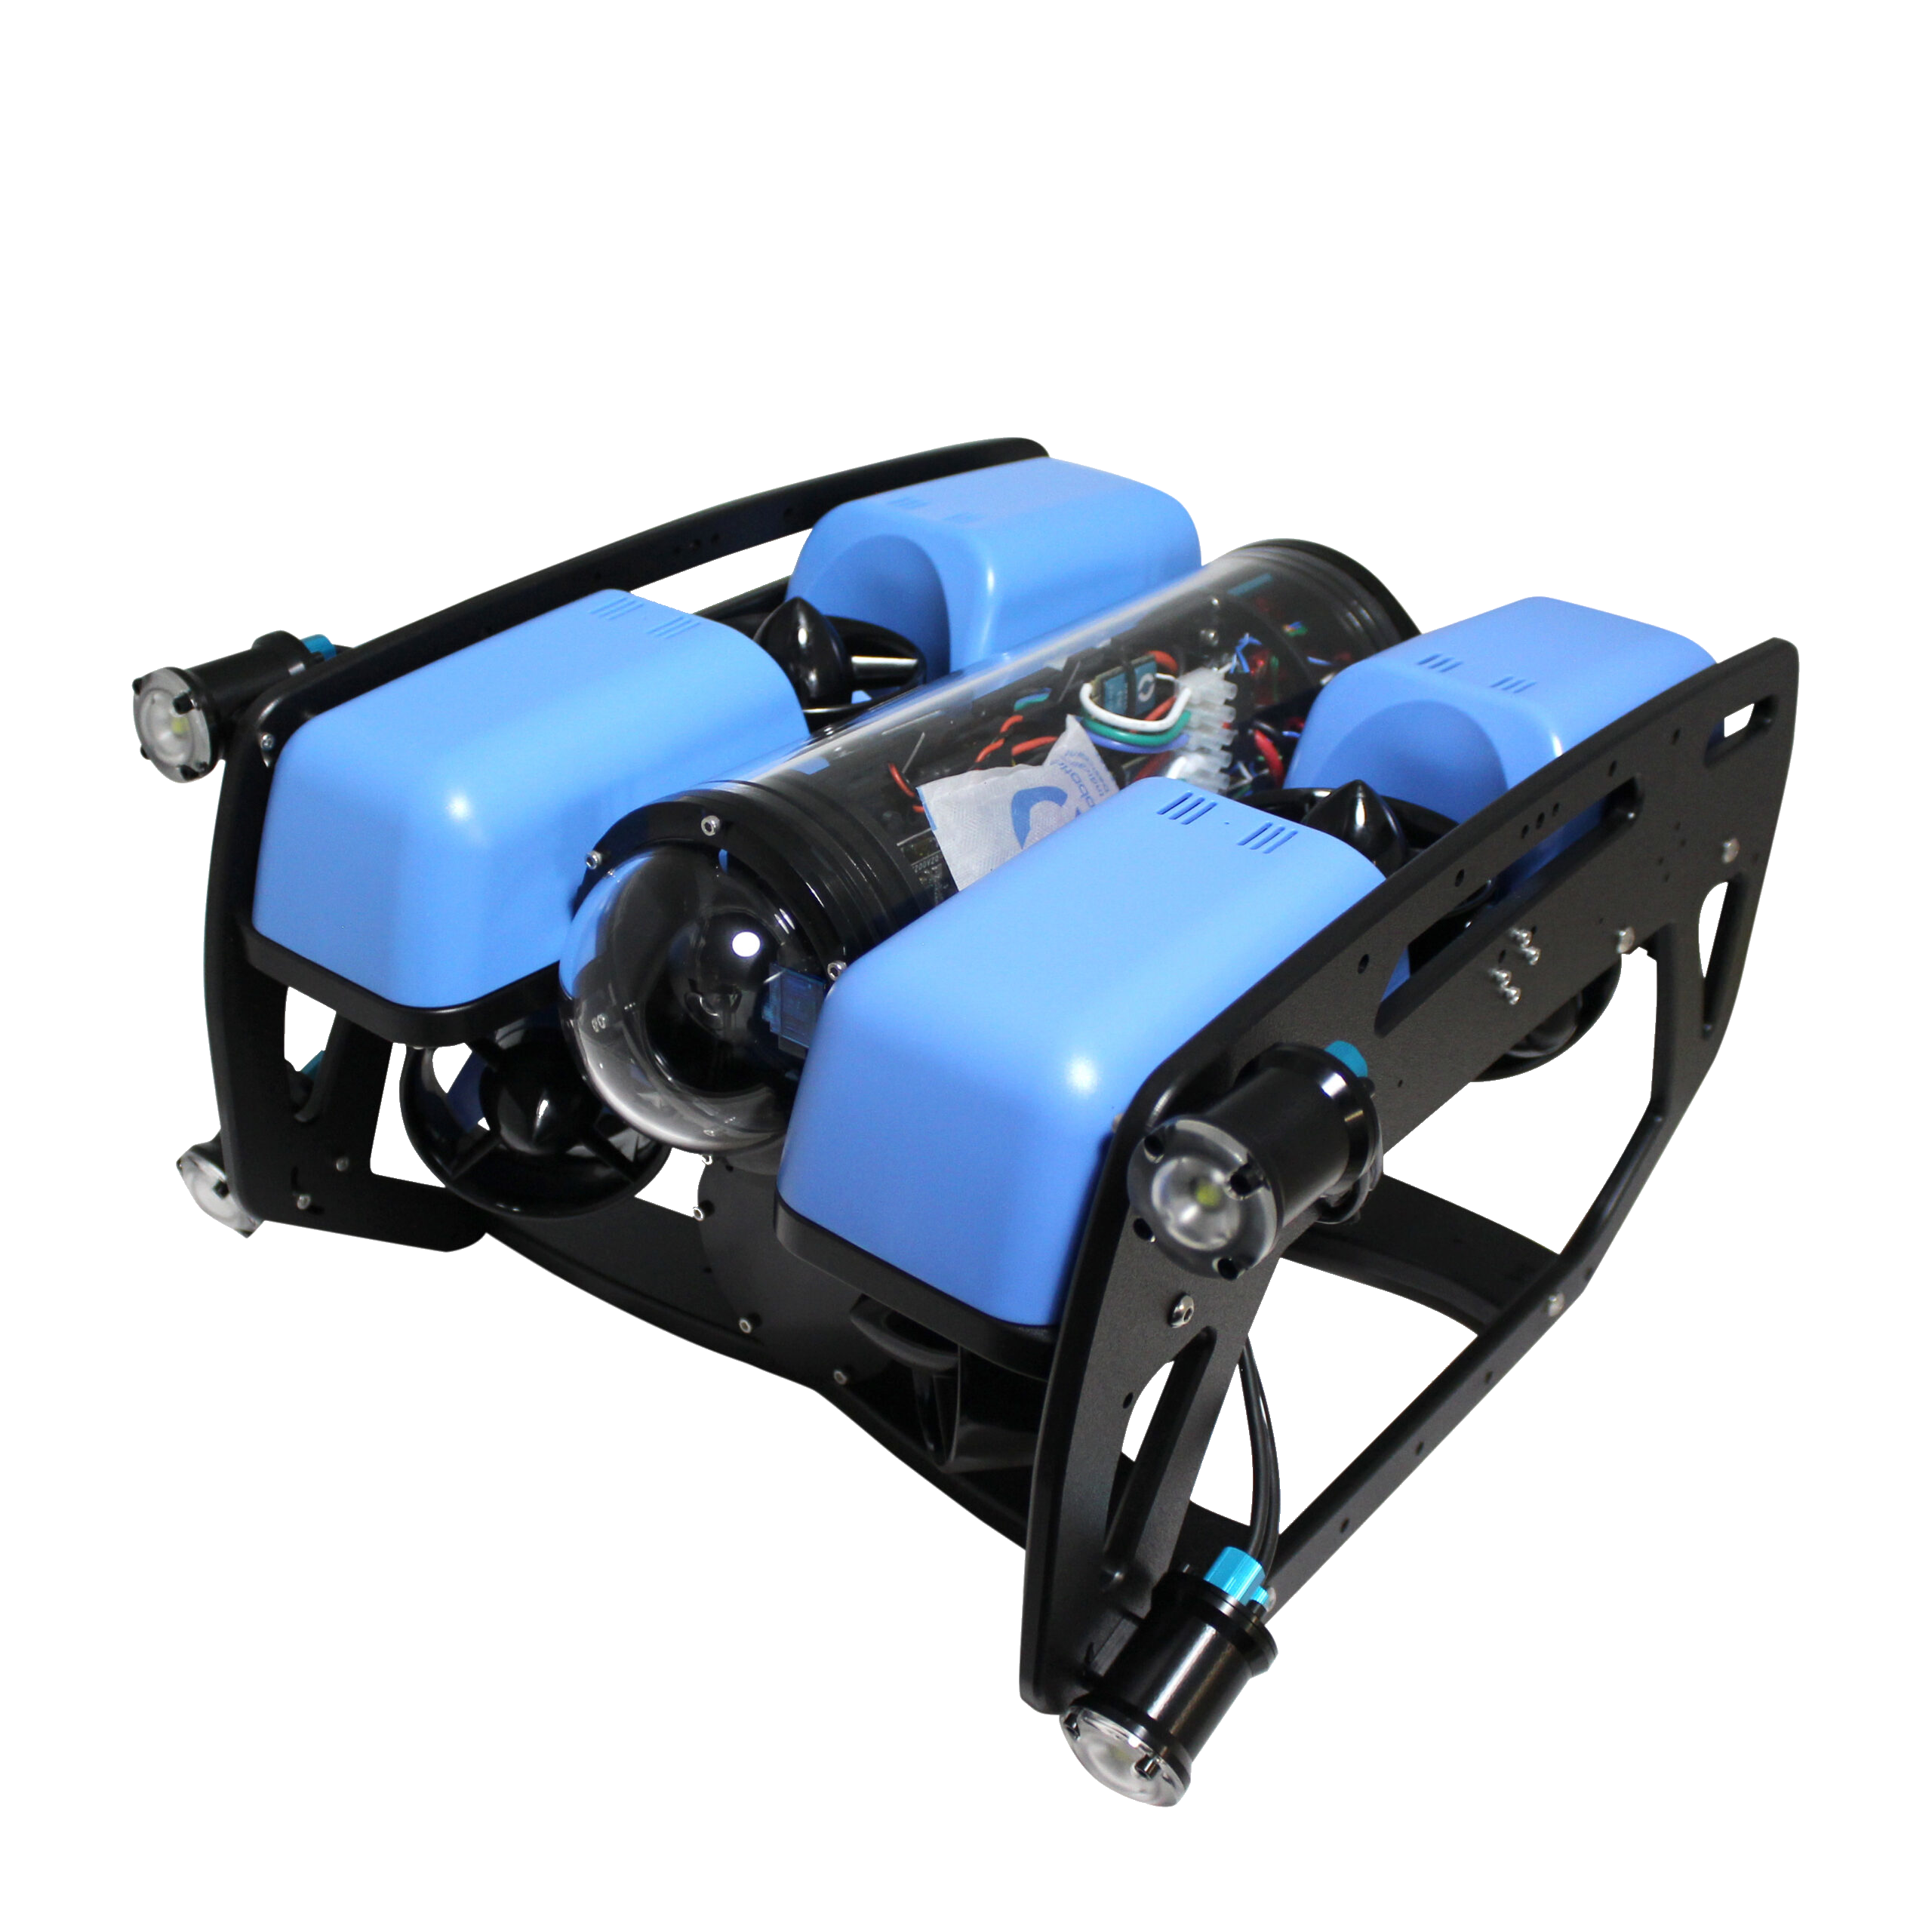
\includegraphics[width=0.8\textwidth]{bluerov.png}
               
               
                  
               
            \end{figure}

            \end{center}
            \column{.33\linewidth}
            \vspace*{0.6cm}
            \begin{center}
          
                \begin{figure}
                    
                    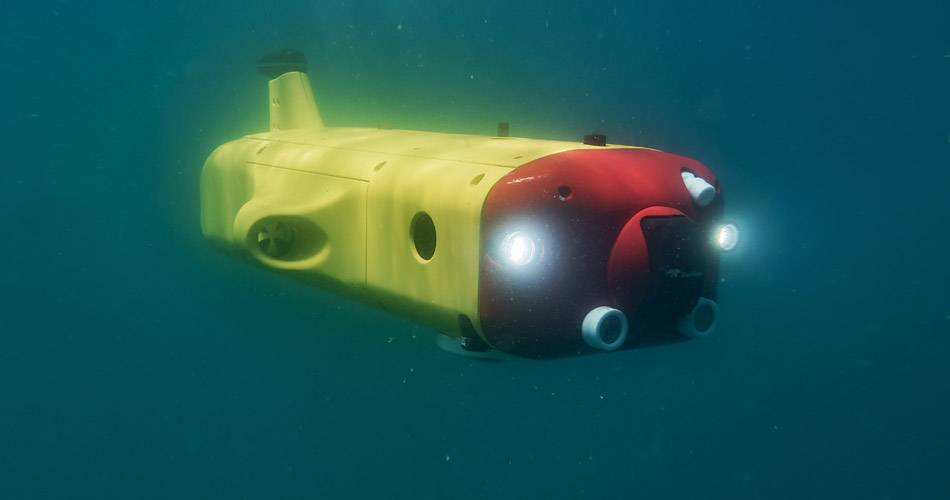
\includegraphics[width=1\textwidth]{flatfish.jpg}
                \end{figure}
            %}
            \end{center}
            
            \column{.33\linewidth}
            \begin{center}
            \vspace*{0.4cm}
            \begin{figure}
                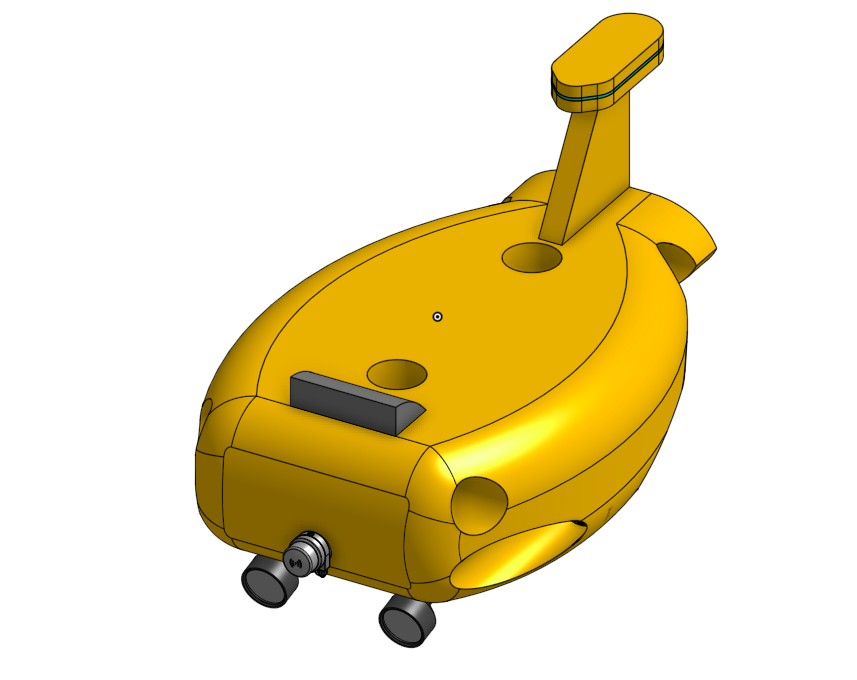
\includegraphics[width=0.8\textwidth]{turbot.png}
            \end{figure}
            \end{center}
        \end{columns}
%*----------- notes
    \note[item]{Notes can help you to remember important information. Turn on the notes option.}
\end{frame}
%-
%*----------- SLIDE -------------------------------------------------------------
\begin{frame}[c]{Objetivo} 
    \framesubtitle{sub-objetivo}
    \transdissolve[duration=0.5]
   
    \begin{center}
        \Wider{%
        \begin{shaded}
        \begin{center}
            \vspace*{0.5cm}
            \resizebox{!}{0.5cm}{%
                \color{bg} The training of researchers in underwater robotics
            }%
        \end{center}
        \end{shaded}
        }%
    \end{center}

\end{frame}
    
   
